\documentclass[a4paper]{report}
\usepackage[utf8]{inputenc}
\usepackage[portuguese]{babel}
\usepackage{hyperref}
\usepackage{a4wide}
\hypersetup{pdftitle={CC - TP01},
pdfauthor={João Teixeira, José Ferreira, Miguel Solino},
colorlinks=true,
urlcolor=blue,
linkcolor=black}
\usepackage{subcaption}
\usepackage[cache=false]{minted}
\usepackage{listings}
\usepackage{booktabs}
\usepackage{multirow}
\usepackage{appendix}
\usepackage{tikz}
\usepackage{authblk}
\usepackage{bashful}
\usepackage{verbatim}
\usepackage{amsmath}
\usepackage{tikz}
\usepackage{tikz,fullpage}
\usepackage{pgfgantt}
\usetikzlibrary{arrows,%
                petri,%
                topaths}%
\usepackage{tkz-berge}
\usetikzlibrary{positioning,automata,decorations.markings}
\AfterEndEnvironment{figure}{\noindent\ignorespaces}
\AfterEndEnvironment{table}{\noindent\ignorespaces}

\begin{document}

\title{LI4 - Proposta de Projeto\\ 
\large PL1 - Grupo 1.1}
\author{José Ferreira (A83683) \and João Teixeira (A85504) \and Miguel Solino (A86435)}
\date{\today}

\begin{center}
    \begin{minipage}{0.75\linewidth}
        \centering
        
\includegraphics[width=0.4\textwidth]{images/eng.jpeg}\par\vspace{1cm}
        \vspace{1.5cm}
        \href{https://www.uminho.pt/PT}
        {\color{black}{\scshape\LARGE Universidade do Minho}} \par
        \vspace{1cm}
        \href{https://www.di.uminho.pt/}
        {\color{black}{\scshape\Large Departamento de Informática}} \par
        \vspace{1.5cm}
        \maketitle
    \end{minipage}
\end{center}

\chapter{Questão 1}

\begin{table}[H]
\begin{tabular}{|l|l|l|l|l|}
\hline
\textit{\begin{tabular}[c]{@{}l@{}}Comando Usado\\ (Aplicação)\end{tabular}} &
  \begin{tabular}[c]{@{}l@{}}Protocolo de\\ Aplicação\end{tabular} &
  \begin{tabular}[c]{@{}l@{}}Protocolo de\\ transporte\end{tabular} &
  \begin{tabular}[c]{@{}l@{}}Porta de\\ atendimento\end{tabular} &
  \begin{tabular}[c]{@{}l@{}}Overhead de transporte\\ em bytes\end{tabular} \\ 
\hline
Ping         & -      & -   & -     & -  \\ \hline
Tracerout    & -      & UDP & 33446 & 8  \\ \hline  
telnet       & telnet & TCP & 23    & 20 \\ \hline 
ftp          & ftp    & TCP & 21    & 20 \\ \hline 
Tftp         & tftp   & UDP & 69    & 8  \\ \hline
browser/http & http   & TCP & 80    & 20 \\ \hline
ssh          & sshv2  & TCP & 22    & 20 \\ \hline
\end{tabular}
\end{table}

\begin{figure}[H]
    \centering 
    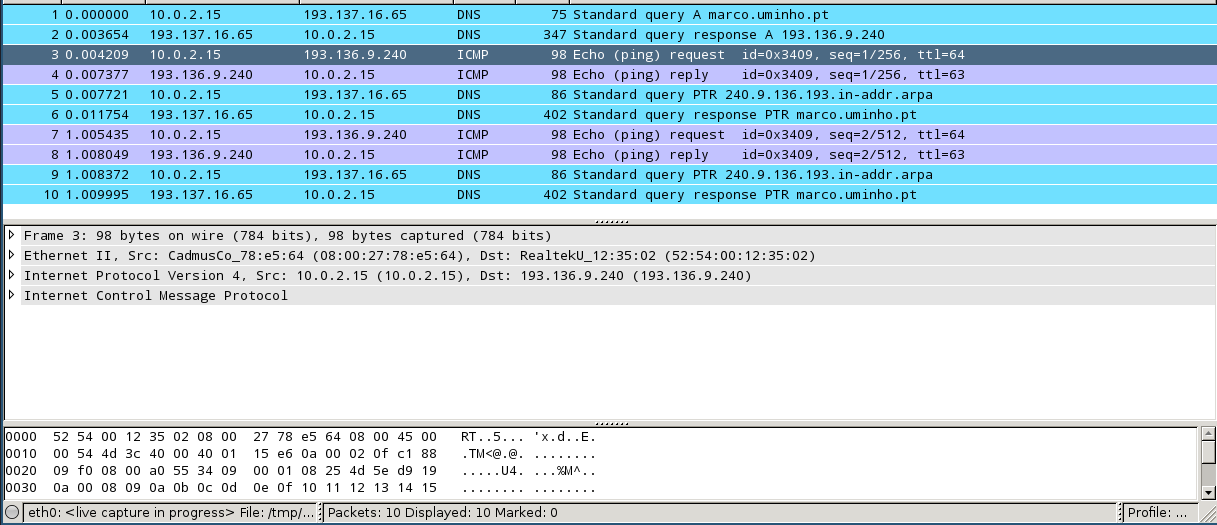
\includegraphics[width=\textwidth]{images/ping.png}  
    \caption{ping}
    \label{fig:ping}
\end{figure}

\begin{figure}[H]
    \centering 
    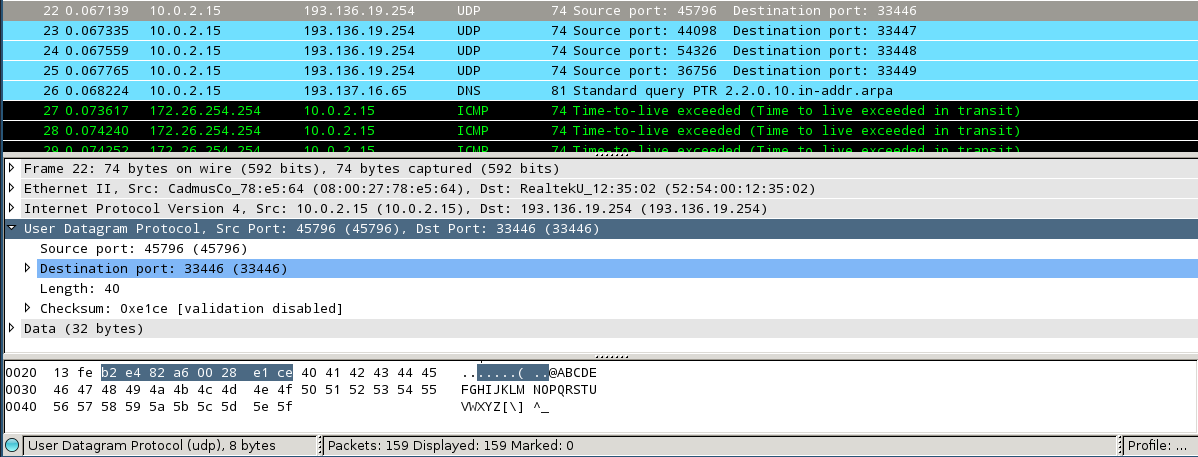
\includegraphics[width=\textwidth]{images/tracerout.png}  
    \caption{tracerout}
    \label{fig:tracerout}
\end{figure}

\begin{figure}[H]
    \centering 
    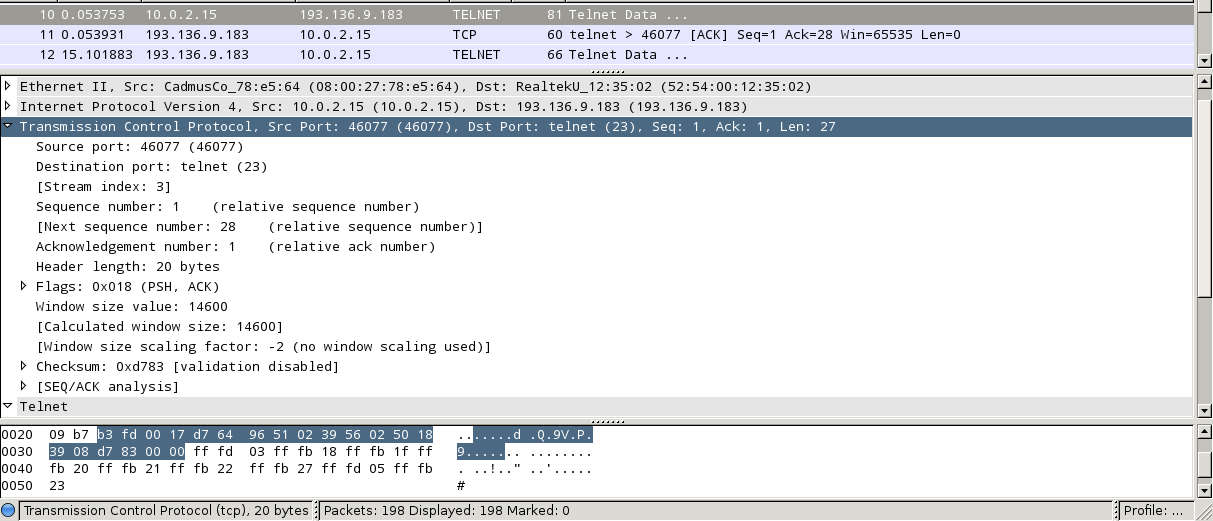
\includegraphics[width=\textwidth]{images/telnet.png}  
    \caption{telnet}
    \label{fig:telnet}
\end{figure}

\begin{figure}[H]
    \centering 
    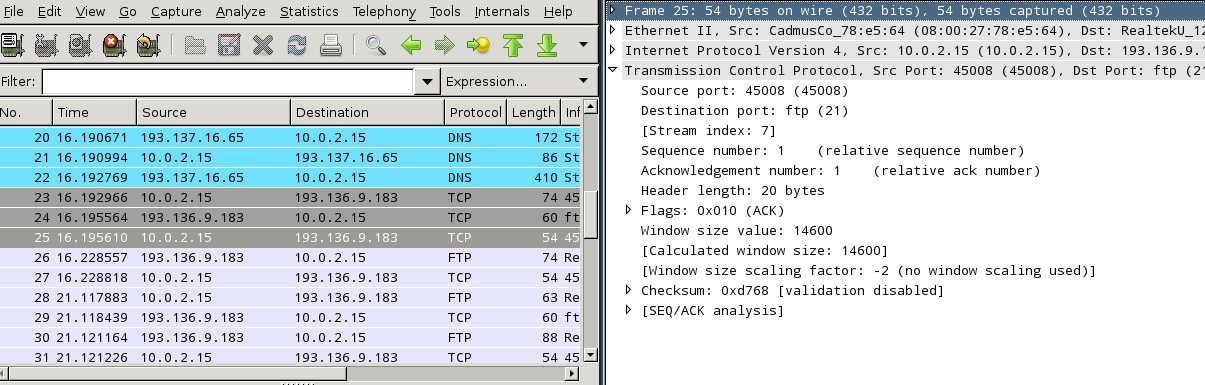
\includegraphics[width=\textwidth]{images/ftp.png}  
    \caption{ftp}
    \label{fig:ftp}
\end{figure}

\begin{figure}[H]
    \centering 
    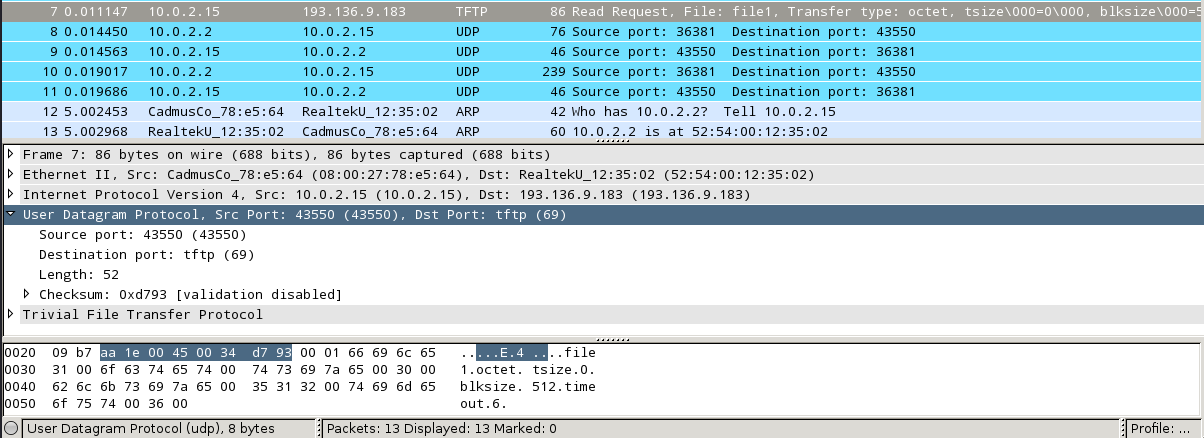
\includegraphics[width=\textwidth]{images/tftp.png}  
    \caption{Tftp}
    \label{fig:tftp}
\end{figure}

\begin{figure}[H]
    \centering 
    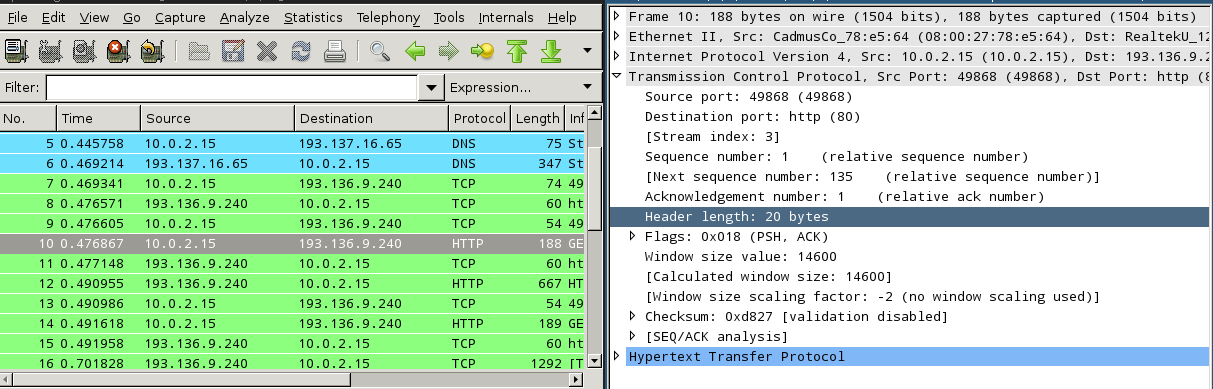
\includegraphics[width=\textwidth]{images/http_browser.png}  
    \caption{http/browser}
    \label{fig:http_browser}
\end{figure}

\begin{figure}[H]
    \centering 
    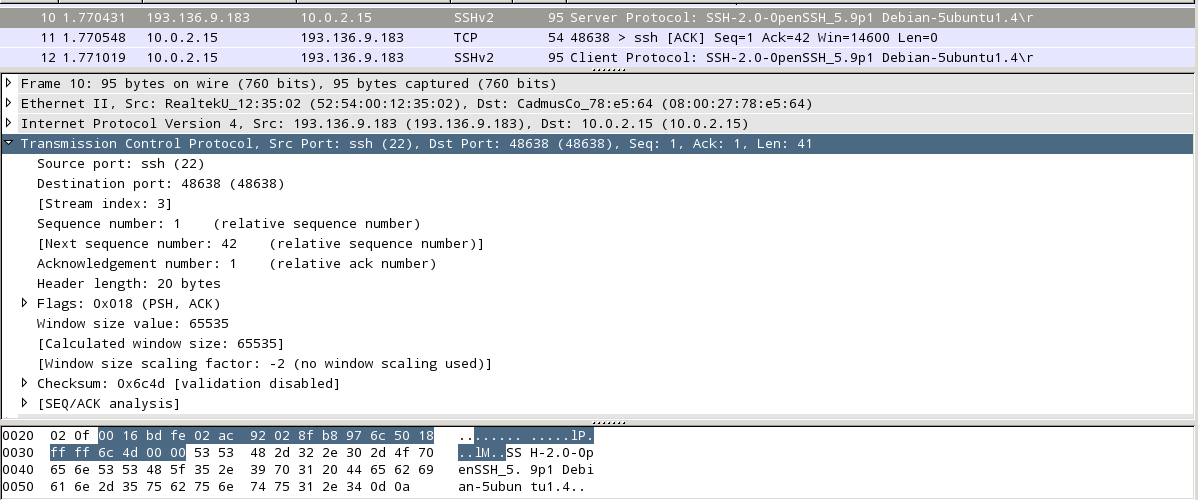
\includegraphics[width=\textwidth]{images/ssh.png}  
    \caption{ssh}
    \label{fig:ssh}
\end{figure}

\begin{figure}[H]
    \centering 
    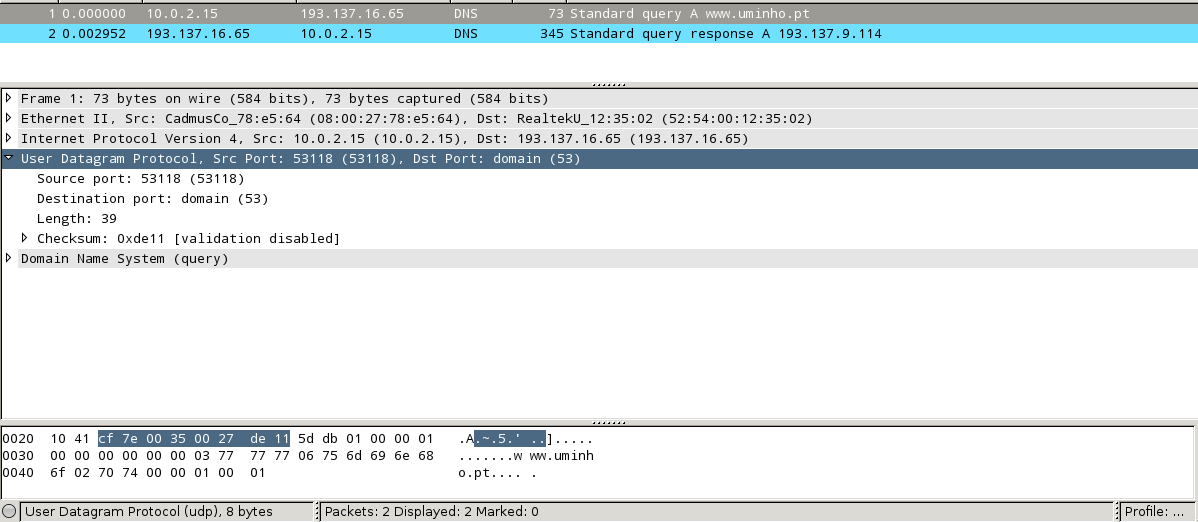
\includegraphics[width=\textwidth]{images/nslookup.png}  
    \caption{nslookup}
    \label{fig:nslookup}
\end{figure}

\chapter{Questão 2}
\begin{figure}[H]
    \centering 
    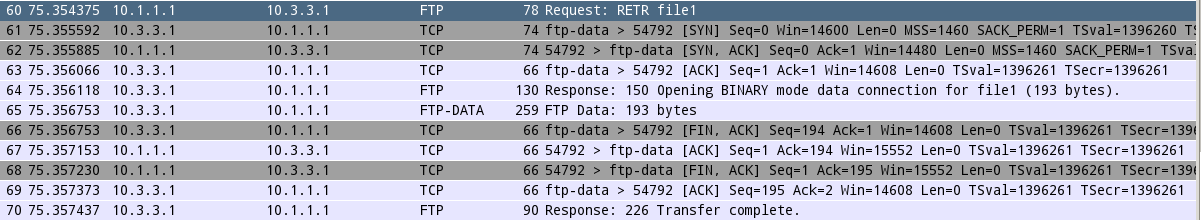
\includegraphics[width=\textwidth]{images/2ftp.png}  
    \caption{ftp}
    \label{fig:2ftp}
\end{figure}

\begin{figure}[H]
    \centering 
    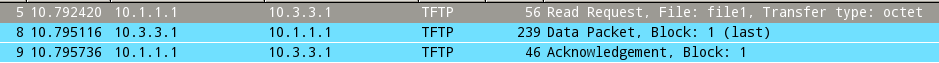
\includegraphics[width=\textwidth]{images/2tftp.png}  
    \caption{tftp}
    \label{fig:2tft:}
\end{figure}

\chapter{Questão 3}


\chapter{Questão 4}
\begin{figure}[H]
    \centering 
    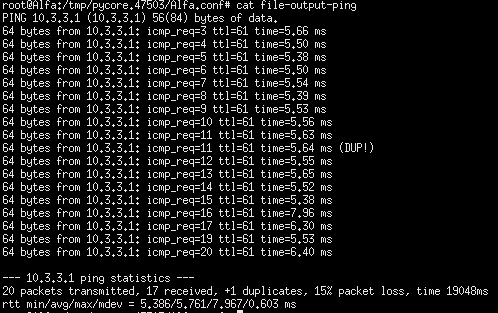
\includegraphics[width=\textwidth]{images/4.png}  
    \caption{4}
    \label{fig:4}
\end{figure}


\end{document}
